
\newcommand{\projectionsWidth}{0.2\textwidth}

\begin{figure}[h]
    \centering
    \bgroup
    \setlength{\tabcolsep}{1mm}
    \def\arraystretch{2}
    \adjustbox{max width=0.92\textwidth}{%
    \begin{tabular}{cccc}
    \multicolumn{4}{c}{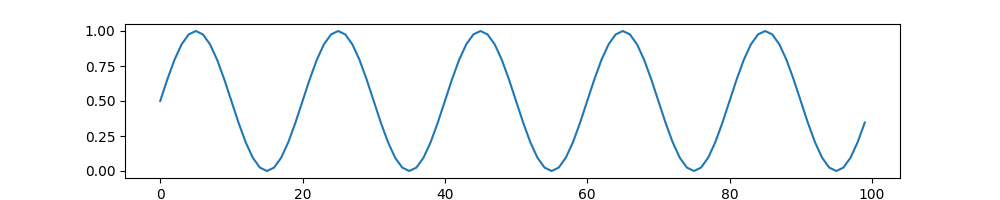
\includegraphics[width=0.95\textwidth, trim={2cm 0cm 2cm 0cm}]{img/projections/signal.png}} \\
        \fbox{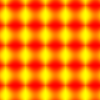
\includegraphics[width=\projectionsWidth]{img/projections/GramianAngularFieldDifference.png}}
         & \fbox{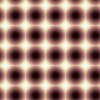
\includegraphics[width=\projectionsWidth]{img/projections/GramianAngularFieldSummation.png}}
         & \fbox{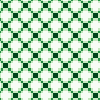
\includegraphics[width=\projectionsWidth]{img/projections/MarkovTransitionField.png}}
         & \fbox{
\includegraphics[width=\projectionsWidth]{img/projections/RecurrencePlot.png}}\\
        \fbox{
\includegraphics[width=\projectionsWidth]{img/projections/PoincatePlotLogarithmGrid.png}}
        & \fbox{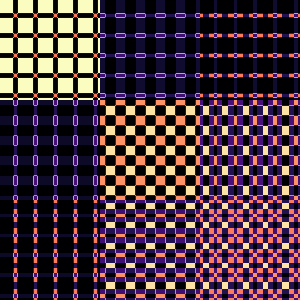
\includegraphics[width=\projectionsWidth]{img/projections/MultiscaleMarkovTransitionField.png}}
        & \fbox{
\includegraphics[width=\projectionsWidth, height=\projectionsWidth]{img/projections/ShortTimeFFT.png}}
        & ~ \\
    \end{tabular}
    }
    \egroup
    \caption{A signal and its various projection obtained by several methods. In the first line, from the left to the right, the methods are: Gramian Angular Diference Field, Gramian Angular Summation Field, Markov Transition Field and Recurrence Plot. The methods of the second line are, from the left to the right: Poincaré Plot Density Map, Multiscale Markov Transition Field and Short Time Fourier Transform Spectogram.}
    \label{fig:literature_projections}
\end{figure}
